%! Author = Saeid Yazdani
%! Date = 7/23/2023


\section{Measurement circuits}
\label{sec:meas-instr}
To have the best control over the output, the system must
guarantee that exact values appearing on the output are measured with confidence
through voltage and current measurement instrumentation and reliably converted
to digital values by high-speed and high-bandwidth \acs{ADC}s.

%%%%%%%%%%%%%%%%%%%%%%%%%%%%%%%%%%%%%%%%%%%%%%%%%%%%%%%%%%%%%%%%%%%%%%%%%%%%%%%%

\subsection{Resistors in Measurement Path}
\label{subsec:shunt-resistor-considerations}

Both voltage and current measurement paths use resistors in dividers
and shunt circuits respectively, and there are multiple critical
factors to consider when selecting the components for these measurement paths.

For voltage measurement, accuracy depends on the precision and
accuracy of the resistors used in the network as ratios are essential
for accurate voltage division.
As the input impedance of the measuring device can affect the divider's
accuracy, high-impedance inputs should be used to minimize loading.

In current-sensing applications, the choice of shunt resistor values has a high
importance as the resistance (\(R_{\text{shunt}}\)) implies the power loss and
voltage drop (\(V_{\text{shunt}}\)).
Reducing the resistance lowers power loss but decreases
voltage drop, affecting current-sensing offset and resolution
\autocite{7384698}.
For voltage divider networks, the resistor values can be more flexible
in a wider range of values, depending on the required voltage division ratio.

As shown in \autoref{fig:resistor-equivalent-circuit}, the package of shunt
resistors can also play a role in measurement quality and measurement bandwidth
due to parasitic inductance and capacitance \autocite{shunt-resistor}.
For the application area of the proposed \acs{DPS}, coaxial shunt resistors are
typically unsuitable for small currents due to their bulkiness, high cost and
parasitics, hence, \acs{SMD} thick film resistors are the preferred
choice \autocite{Costa}.

\begin{figure}[h]
    \centering
    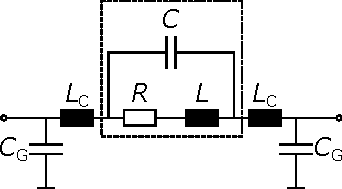
\includegraphics[width=0.5\textwidth]
    {figures/prototype/resistor-equivalent-circuit}
    \caption[Equivalent circuit]{
        Equivalent circuit of a resistor \autocite{vishay:thinfilm} where:
        \emph{$R$:} nominal resistance,
        \emph{$C$:} internal shunt capacitance,
        \emph{$L$:} internal inductance,
        \emph{$L_C$:} external connection inductance,
        \emph{$C_G$:} external connection capacitance to ground.
    }
    \label{fig:resistor-equivalent-circuit}
\end{figure}

In high-frequency current sensing, minimizing parasitic inductance is crucial
to avoid phase shifts or delays in the measurement while in
voltage divider networks, \emph{parasitic capacitance} can affect the accuracy
at high frequencies or high-impedance networks.
Therefore special shunt resistors with low inductance and capacitance are used.

\ac{TCR} describes how a resistor changes over temperature, measured
in \SI{}{\ppm\per\kelvin}.
This change in resistance is reversible when the temperature returns to normal,
as long as the internal structure hasn't been permanently altered by extreme
heat from a strong pulse or overload.

A low \acs{TCR} ensures that the resistor remains stable across
a range of temperatures, providing more accurate and reliable measurements
since any change due to temperature fluctuations can lead to significant
errors in the measured current or voltage \autocite{vishay:tcr}.

%%%%%%%%%%%%%%%%%%%%%%%%%%%%%%%%%%%%%%%%%%%%%%%%%%%%%%%%%%%%%%%%%%%%%%%%%%%%%%%%

\subsection{The Voltage Measurement}
\label{subsec:voltage-emasurement}
Using resistor divider networks is a common way of measuring voltage as
the voltage readings at the resistor network junction should be
proportional to the true input voltage applied~\autocite{1608605}.

There are 5 voltage ranges provisioned for the system and
\autoref{fig:voltage-sense-divider-network} shows the simplified overview of
the implemented divider network using \acsp{SSR} for range selection.

\begin{figure}[h]
    \centering
    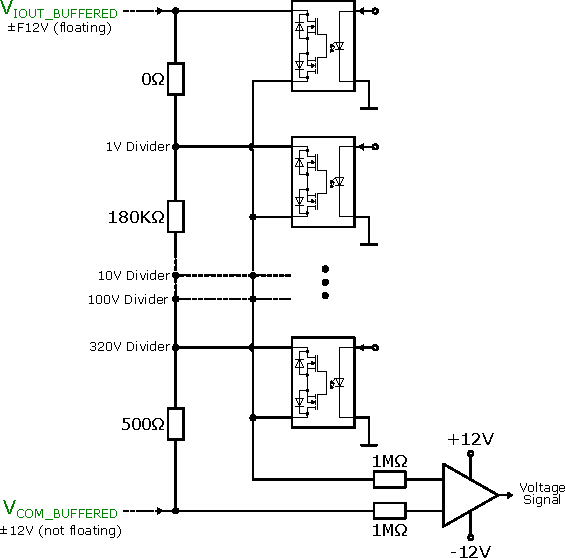
\includegraphics[width=0.8\textwidth]
    {figures/prototype/voltage-sense-divider-network}
    \caption[Voltage-Sense Divider Network]{
        Simplified overview of the voltage measurement divider network.
        The input voltage is isolated and buffered before being fed into
        the divider network as sketched in
        \autoref{fig:input-buffering-and-guarding}.
    }
    \label{fig:voltage-sense-divider-network}
\end{figure}


Any resistive divider at the driver output introduces an error current, and we
need an error cancellation scheme even in the case of \acs{FET}-based
sensing.
Therefore, as shown in \autoref{fig:input-buffering-and-guarding}, an
electrometer amplifier (\emph{ADA4530}) is used to buffer the voltage signal to
prevent loading effects because of its high
\SI{100}{\tera\ohm}
input resistance and input bias currents in the \SI{}{\femto\ampere}
range \autocite{ada4530}.

A disadvantage of having no initial load at the output (due to
the electrometer amplifier) is capacitive
crosstalk via open relays on the output connector as shown in
\autoref{fig:frontend-board}.
Any step at the driver output will be seen as a
step at the source output because there is a capacitive transfer function.
For $C_{load} = 0$, we get a transfer function $H = 1$, i.e. we find the
step at the output, and for $C_{load} >> C_{relay}$, we get an indirect
proportionality.
Additional guard amplifiers are used to minimize this effect.

\begin{figure}[h]
    \centering
    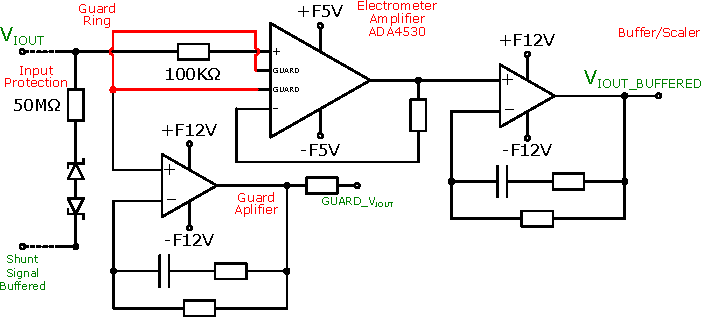
\includegraphics[width=\textwidth]
    {figures/prototype/input-buffering-and-guarding}
    \caption[Input Buffering and Guarding]{
        A femtoampere electrometer amplifier is used for buffering
        input signals fed to the voltage divider network. A similar
        arrangement is also used for current measurement circuit.
        The integrated guard ring in \emph{ADA4530} minimizes leakage currents
        and prevent parasitic capacitance \autocite{ada4530}.
    }
    \label{fig:input-buffering-and-guarding}
\end{figure}

There are multiple floating supplies available in the system and these supplies
are also used for the voltage and current buffers which feed both measurement
circuit inputs.

In a fault situation, there may be a large differential voltage across
the current sense resistors, and we need to protect the input of the sense
amplifier. A series resistor and two diodes offer protection as shown
in \autoref{fig:input-buffering-and-guarding}.

To keep power dissipation in the floating supply generator
low, we use special buffer amplifiers with low supply currents
and input bias current smaller than \SI{10}{\pico\ampere}.

%%%%%%%%%%%%%%%%%%%%%%%%%%%%%%%%%%%%%%%%%%%%%%%%%%%%%%%%%%%%%%%%%%%%%%%%%%%%%%%%

\subsection{The Current Measurement}
\label{subsec:current-emasurement}

There are a total of 10 ranges provisioned in the system
in the range of \SI{10}{\nano\ampere} to \SI{10}{\ampere} in multiples of 10.
As shown in \autoref{fig:current-sense-shunt-chain}, current measurement is
based on high-side sensing and the current range is selected via
electronic switches.
The exact values of shunt resistors used in the prototype and their properties
are presented in \autoref{table:current_sense_resistors}.

\begin{figure}[h]
    \centering
    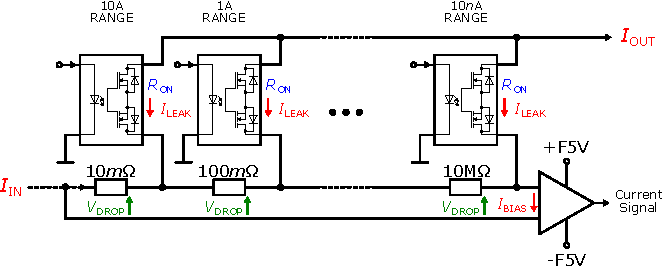
\includegraphics[width=\textwidth]
    {figures/prototype/current-sense-shunt-chain}
    \caption[Current-Sense Shunt Chain]{
        Simplified overview of the current sensing circuit and
        corresponding shunt resistors chain where voltage drops
        over shunt resistors, on-state
        resistance and off-state leakage current with resulting bias
        current into the current sense amplifier are annotated.
        The total resistance for each range is the sum of all
        shunt resistors of the previous ranges.
    }
    \label{fig:current-sense-shunt-chain}
\end{figure}

\begin{table}[h!]
    \centering
    \begin{tabular}{|l|c|c|c|}
        \hline
        \textbf{Range}             & \textbf{Resistor Value} & \textbf{Current}         & \textbf{Accuracy}       \\ \hline
        \SI{\pm10}{\ampere}        & \SI{10}{\milli\ohm}     & \SI{5.75}{\milli\ampere} & \SI{23}{\milli\ampere}  \\ \hline
        \SI{\pm1}{\ampere}         & \SI{100}{\milli\ohm}    & \SI{325}{\micro\ampere}  & \SI{1.3}{\milli\ampere} \\ \hline
        \SI{\pm100}{\milli\ampere} & \SI{1}{\ohm}            & \SI{32.5}{\micro\ampere} & \SI{130}{\micro\ampere} \\ \hline
        \SI{\pm10}{\milli\ampere}  & \SI{10}{\ohm}           & \SI{2}{\micro\ampere}    & \SI{8}{\micro\ampere}   \\ \hline
        \SI{\pm1}{\milli\ampere}   & \SI{100}{\ohm}          & \SI{200}{\nano\ampere}   & \SI{0.8}{\micro\ampere} \\ \hline
        \SI{\pm100}{\micro\ampere} & \SI{1}{\kilo\ohm}       & \SI{20}{\nano\ampere}    & \SI{80}{\nano\ampere}   \\ \hline
        \SI{\pm10}{\micro\ampere}  & \SI{10}{\kilo\ohm}      & \SI{2}{\nano\ampere}     & \SI{8}{\nano\ampere}    \\ \hline
        \SI{\pm1}{\micro\ampere}   & \SI{100}{\kilo\ohm}     & \SI{325}{\pico\ampere}   & \SI{1.3}{\nano\ampere}  \\ \hline
        \SI{\pm100}{\nano\ampere}  & \SI{1}{\mega\ohm}       & \SI{133}{\pico\ampere}   & \SI{530}{\pico\ampere}  \\ \hline
        \SI{\pm10}{\nano\ampere}   & \SI{10}{\mega\ohm}      & \SI{27}{\pico\ampere}    & \SI{110}{\pico\ampere}  \\ \hline
    \end{tabular}
    \caption[Current Sense Shunt Resistors]{
        Current ranges and associated shunt resistor and switch properties for
        each range.
    }
    \label{table:current_sense_resistors}
\end{table}

Selecting the
right type of switch and its properties for each current range is a challenging
task.
Besides cost and reliability, critical decision factors for selecting the
right type of switching component are:

\begin{itemize}[topsep=8pt,itemsep=4pt,partopsep=4pt, parsep=4pt]

    \item \textbf{On Resistance(\(R_{ON}\)):} All relays, including
    \acp{SSR} exhibit a series resistance.
    This resistance must be as low as possible.
    The On Resistance should also be stable for different temperatures.

    \item \textbf{Leakage Current:} During off-state, there will be a current
    leakage across the switch terminals.
    This value should be less than the desired accuracy.

    \item \textbf{Switching Speed:} When tracking \ac{DUT} power, the
    system may need to switch between lower or higher current or voltage
    ranges.
    The switches must be fast enough to follow the change quickly.

    \item \textbf{Electrical Isolation:} The switch must be able to withstand
    the desired electrical isolation in the range of a few
    \SI{}{\kilo\volt}.

    \item \textbf{Current Rating:} The switches must safely handle the
    current through them.

\end{itemize}

For the above reasons, the switches of choice were from the
\emph{OptoMOS\texttrademark} family of \acp{SSR} that exhibit better
characteristics such as switching speed, cost and reliability than other
options such as reed relays.

If the output of the floating current sense amplifier includes a floating
voltage component, which is not referenced to the same ground as the subsequent
circuitry (e.g. ADC), subtraction will be necessary
as floating current sense amplifiers deliver floating output voltages,
i.e. \( V_{\text{out}} = V_{\text{float}} + V_{\text{signal}} \), there will be
a need to extract the signal by a subtraction:
\( V_{\text{signal}} = V_{\text{out}} - V_{\text{float}} \).
For \(|V_{\text{float}}| > 10 \, \text{V}\), we cannot use simple op amp
circuitry and we need to scale voltages to acceptable levels:


\begin{equation}
    V_{\text{signal}} = K \left( \frac{V_{\text{out}}}{K} - \frac{V_{\text{float}}}{K} \right)
    \quad \text{where} \quad
    \left| \frac{V_{\text{out}}}{K} \right| \leq 10 \, \text{V}, \quad
    \left| \frac{V_{\text{float}}}{K} \right| \leq 10 \, \text{V}
\end{equation}


%%%%%%%%%%%%%%%%%%%%%%%%%%%%%%%%%%%%%%%%%%%%%%%%%%%%%%%%%%%%%%%%%%%%%%%%%%%%%%%%

\subsection{\acs{ADC} Interfacing}
\label{subsec:adc-interfacing}

As stated in \autoref{sec:system-overview}, the resulting voltage and current
signals in the measurement circuit will be fed into the FPGA for control
loop processing over \acs{LVDS} interface.

Since the results of voltage divider and current shunt networks are single-ended
analog signals, they need to be converted into differential signals using a
converter such as LT6350 \autocite{ad:lt6350} as the \ac{ADC} chip used in
the design requires two complementary signals to improve noise rejection and
accuracy.

The resulting differential signal is fed into the \acs{ADC}, \emph{LTC2386}
that is a 16-bit, high-speed \acs{SAR} \acs{ADC}
\autocite{ad:ltc2386}.
The interfacing circuit is presented in \autoref{fig:adc-input-interface}.

\begin{figure}[h]
    \centering
    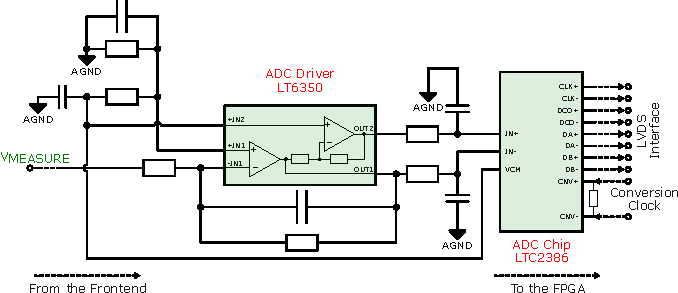
\includegraphics[width=\textwidth]
    {figures/prototype/adc-input}
    \caption[ADC Input Interface]{
        Equvivalent circuit for interfacing the voltage measurement signal
        to the FPGA.
        The current measurement signal follows the same procedure except
        using an \ac{LVDS} isolator for further reducing ground loops and noise.
    }
    \label{fig:adc-input-interface}
\end{figure}


%%%%%%%%%%%%%%%%%%%%%%%%%%%%%%%%%%%%%%%%%%%%%%%%%%%%%%%%%%%%%%%%%%%%%%%%%%%%%%%%

\subsection{\acs{DAC} Interfacing}
\label{subsec:dac-interfacing}

After data processing by the \acs{FPGA}, the resulting \emph{coarse} and
\emph{vernier} as well as the desired \emph{setpoint} must be fed into the
driver stage.

There are three \acs{DAC} chips on the controller board to generate
analog signals from digital results and the \acs{FPGA} drives the
16-bit, high-speed (50\acs{MSPS}) \acs{DAC} directly using \acs{GPIO} outputs.

All three DAC chips are powered by \SI{\pm5}{\volt} supplies to allow for an
output swing around ground level in order to be fed into the conditioning
amplifier for voltage translation.

\autoref{fig:dac-output-interface} illustrates the circuit used for
generating analog signals from the \ac{FPGA}'s output pin.
All three DACs in the system follow the same principle.

\begin{figure}[h]
    \centering
    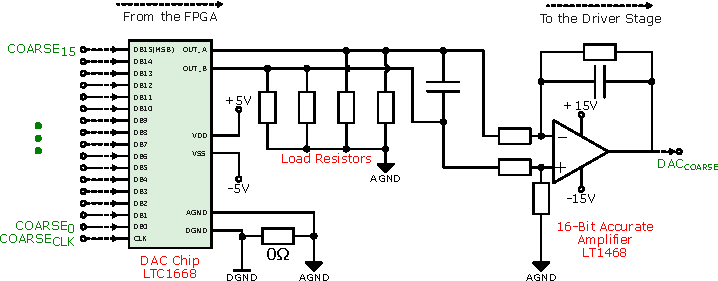
\includegraphics[width=\textwidth]
    {figures/prototype/dac-output}
    \caption[DAC Output Interface]{
        Conversion of \emph{coarse} digital value into an analog signal.
        The load resistors on the DAC
        produce a differential output voltage without degrading the converter's
        linearity \autocite{ad:lt1668}.
    }
    \label{fig:dac-output-interface}
\end{figure}







